\begin{center}
	
	\begin{tabular}{rp{16cm}lp{20cm}}%{rl}
		
		% after \\: \hline or \cline{col1-col2} \cline{col3-col4} ...
		
		论文地址:& \href{https://dl.acm.org/doi/pdf/10.1145/3350546.3352513}{https://dl.acm.org/doi/pdf/10.1145/3350546.3352513} \\
		来源:& WI, 2019 \\
		作者:& Hiromi Nakagawa, et al. \\
		单位:& The University of Tokyo$_{\times 3}$ \\
		源码:& \href{https://github.com/jhljx/GKT}{GKT} \\
		
		%  slides:& \href{http://yunshengb.com/wp-content/uploads/2017/03/nips_2018_r2l_workshop_talk.pdf}{{\footnotesize Convolutional Set Matching for Graph Similarity}}\\
		
		关键词:& \textbf{Knowledge Tracing, GNN} \\
		
		写于:& \date{2021-09-22}
		
	\end{tabular}
	
\end{center}

该论文\cite{nakagawa2019graph-based}将课程表达为一个Graph,将知识追踪问题转化为时间序列的结点分类问题,并提出了Graph-based Knowledge Tracing(GKT)。

\paragraph{问题定义}
从课程的组成结构来看,更像是一个有向图的结构,图中的结点是知识点,边表示知识点之间的依赖关系。 以往的Knowledge Tracing模型并没有考虑课程潜在的graph结构。 

GKT将一个课程(coursework)的知识分解为一定数量的知识概念,以知识概念作为结点,概念之间的依赖关系作为边构建graph。学生的知识水平是以其对课程中知识点的掌握程度/熟练程度来衡量的。一个学生与某个知识点进行交互,影响的不只是该知识点,还有依赖于该知识点的知识点和该知识点依赖的知识点。

但是在现实中,课程的图结构并不是显示存在的。\textbf{如何获得课程的图结构呢?}一种简单的思路是,依据数据中知识点的统计信息构建图;另一种思路是,通过一些基础的任务来学习出图的结构,这其中就涉及到GNN中的边特征学习。

形式化定义一下:
一门课程表示为:$G = (V, E),\:\: V=\{v_1, ..., v_N\},\:\: E \subseteq V\times V$。$V$表示课程所包含的$N$个知识点,$E$表示知识点之间的依赖关系。论文中假设学生对知识点的掌握是动态的:用$\boldsymbol{h}^t = \{\boldsymbol{h}^t_{i \in V}\}$表示学生在$t$时的知识状态。当学生与一个结点交互时,该结点及其一阶邻居的$\boldsymbol{h}$都会被更新。



\paragraph{GKT}
GKT的流程如Fig.\ref{fig:gkt}所示。GKT的关键有二:1)工作流程;2)如何得到隐式的课程graph。
\begin{figure}[h]
	\centering
	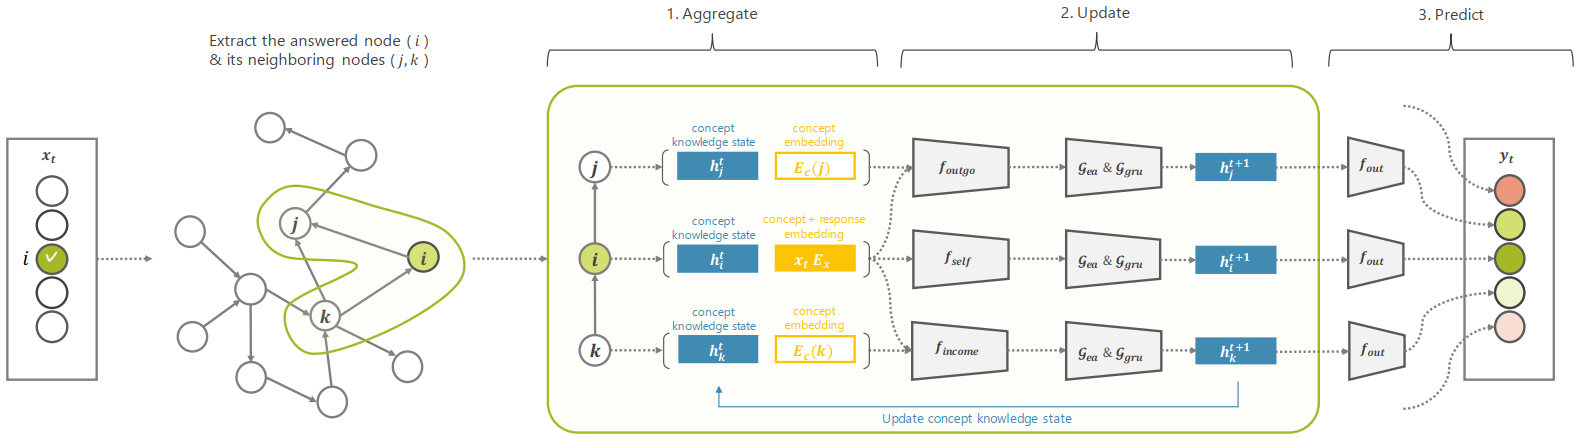
\includegraphics[width=.9\textwidth]{pics/gkt.png}
	\caption{GKT流程}
	\label{fig:gkt}
\end{figure}

\subparagraph{工作流程}结点的更新缘自学生的与课程的交互。流程分为三步走:
\begin{enumerate}
	\item Aggregates:根据$t$时的交互汇集相关结点的$\boldsymbol{h}^t_{i}$。交互表示为:$\boldsymbol{x}_t \in \{0, 1\}^{2N}$,表示的含义为交互的知识点和学生的答案
	\item Update:将汇集后的结点状态进行转换后输入到GRU中得到结点$t+1$时的$\boldsymbol{h}^{t+1}$
	\item Predict:基于$\boldsymbol{h}^{t+1}$预测学生对每个知识点进行回答时正确的概率
\end{enumerate}
工作流程比较常规,与结点预测任务的流程基本一样。

\subparagraph{隐式的图结构}因为课程的graph结构是静态的,因此如何得到隐式结构也就等于如何得到邻接矩阵$\boldsymbol{A}$。论文中给出了两种方法。
\par{Statistics-based Approach} 从数据的统计信息中得到邻接矩阵,论文中给出了三种构建的方法,不赘述。
\par{Learning-based Approach} 学习的方法重点也是在如何得到邻接矩阵,只不过矩阵中的值是在学习过程中得到的,也不赘述。

论文采用的数据集:\href{https://sites.google.com/site/assistmentsdata/home/assistment-2009-2010-data/skill-builder-data-2009-2010}{ASSISTments}和\href{https://pslcdatashop.web.cmu.edu/KDDCup/}{KDDCup-2010},指标是AUC。

\paragraph{总结}

\begin{itemize}
	\item 基于图结构、知识点随时间变化的状态表示学生的知识水平
	\item 支持多种方式得到隐式的图结构
	\item 如何得到知识点和回答的Embedding没有在文中解答
	\item 不同的学生学习同一门课程时使用的是相同的课程graph,但是如何针对每个学生给出初始的结点状态、训练样本是如何构造的没有详细描述
\end{itemize}

